\section{Methods}
We developed CEMRG Heartbuilder, a pipeline for the streamlined creation of simulation-ready meshes, 
generated from a CT scan. 
The pipeline to process the CT scans is based on the work by~\cite{strocchi2020_cohort} 
but streamlined into a single integrated workflow.
Processing of the information consisted of three stages: 
image to mesh analysis, consisting of a multi-stage segmentation (Section~\ref{sec:segmentation}), 
upsampling, and mesh generation (Section~\ref{sec:meshing}); 
mesh processing and model creation, which includes the assignment of fibre orientations
in the ventricles and atria, 
and the tagging of the mesh with the different labels needed for the simulations (Section~\ref{sec:model-creation}); 
and simulations. 
The multi-stage segmentation and mesh extraction substages are open source, 
whilst some of the mesh post-processing and simulation stages use the 
cardiac arrhythmia research package (CARP)~\cite{carp-2003}. 
Note that the modular structure of the CEMRG Heartbuilder allows for third-party projects to be 
included to be made completely open source.

\subsection{Image to Mesh Stage}
\subsubsection{Multi-stage Segmentation}\label{sec:segmentation}
The image to mesh stage consists of a segmentation of the CT scan via the 
deep learning model by~\cite{hao2021_ccta}, Figure~\ref{fig:methods-segmentation}a, 
which identifies 10 distinct regions: 
left ventricle myocardium, and blood pools of the left and right ventricles, the left and right atrium, 
the pulmonary artery, the aorta, 
the left and right atrial pulmonary veins, and left atrial appendage. 
Regions are marked in the segmentation with different integer values,
we refer to these as ``labels'' throughout the manuscript.
% The segmentation is a multi-stage process involving training different U-Nets 
% and refining the output of each to produce the final image-to-label 3D U-Net 
% (Figure~\ref{fig:methods-segmentation}a). 
The user then identifies the different labels in the U-Net output, which splits the pulmonary veins 
into the superior and inferior veins. 
The user selects two sets of 3~points to identify the location and orientation of 
the superior and the inferior venae cavae.
A post-processing stage follows, increasing the number of labels to 37 (Figure~\ref{fig:methods-segmentation}b). 
This stage creates the myocardia, valve planes, and vein rings. 
The myocardia of the right ventricle (\RV), the atria, the aorta and pulmonary artery are extracted
through the use of distance maps, with a user-selected thickness of 3.5mm for the \RV, and 
2mm for the remaining structures and coupling the different regions to ensure no overlap occurs.
A table of the labels is provided in the Supplementary material.
% See the Supplementary material for a detailed explanation of these points' locations and 
% of the evolution of the segmentation as the post-processing stage occurs.

\begin{figure}[hbpt]
    \centering
    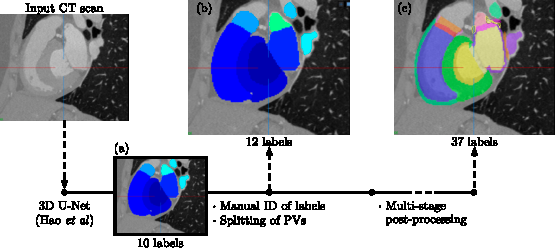
\includegraphics[width=\textwidth]{pics/methods-segmentation.pdf}
    \caption{
        \textbf{Multi-stage segmentation process. }
        CemrgApp uses the deep learning model developed by \cite{hao2021_ccta} to segment the heart. 
        (a) The output of the U-Net model, which identifies 10 regions, or ``labels'', 
        as described in the text.
        (b) The output of the intermediate stage, where the user manually 
        splits the pulmonary veins into superior and inferior \added[id=R1, comment={R1-Min-1: Figure 2 Visual Distinction}]{(marked by contrasting colours)}.
        (c) The final output of the post-processing stage, where the myocardium of the different structures
        is extracted, increasing the number of labels to 37.
        The final segmented images are then upsampled to an isotropic resolution of 0.1mm and 
        smoothed.
    }
    \label{fig:methods-segmentation}
\end{figure}

CemrgApp aggregates the different workflows through a combination of code running natively on the app and 
a docker wrapper, which calls the segmentation and different post-processing stages. 
The image analysis stage finalises by upsampling the 37-label segmentation to an isotropic resolution of 0.15mm, 
and a applies a smoothing algorithm~\cite{crozier2016_segsmooth}. 

\subsubsection{Conversion to Mesh}\label{sec:meshing}
A volumetric mesh is extracted from the smooth segmentation using a meshing tool developed in-house, 
which comes packaged with CemrgApp and is based on the Computational Geometry Algorithm Library (CGAL)~\cite{cgal}. 
\added[id=R2, comment={R2-2a, R2-5: Element type and mesh density control}]{
    The CGAL mesher generates unstructured volumetric meshes 
    composed of linear tetrahedral elements (4 nodes per element). Target 
    element edge length was set to approximately 0.5~mm via the 
    \texttt{cell\_size} and \texttt{facet\_size} parameters. 
    Mesh density is controlled via CGAL parameters 
    (\texttt{facet\_size}, \texttt{cell\_size}, \texttt{facet\_distance}), 
    which are specified globally for the entire heart geometry. Complete 
    parameter specifications are provided in the Supplementary Material.
}
The next step is to extract the myocardia, simplify the mesh topology, and relabel the tags using 
meshtool~\cite{Neic2020-meshtool}.
The simplification consists in identifying elements insufficiently connected to neighbours of the same class.
% The element tags of the entire volumetric mesh are cleaned up and relabelled 
% with meshtool~\cite{Neic2020-meshtool}, before removing the blood pools.
A complete description of the CGAL parameters, which can be modified by the user, 
is available in the Supplementary material. 
Figure~\ref{fig:methods-mesh} shows the output of the meshing process from the smooth segmentation 
to the working mesh re-labelled and with the blood pools removed.
\added[id=R2, comment={R2-2b: Final mesh statistics}]{
    The final simulation-ready models contained a mean of $2.6 \times 10^6$ elements per heart 
    (range $1.9$--$4.5 \times 10^6$).
}

\begin{figure}[hbpt]
    \centering
    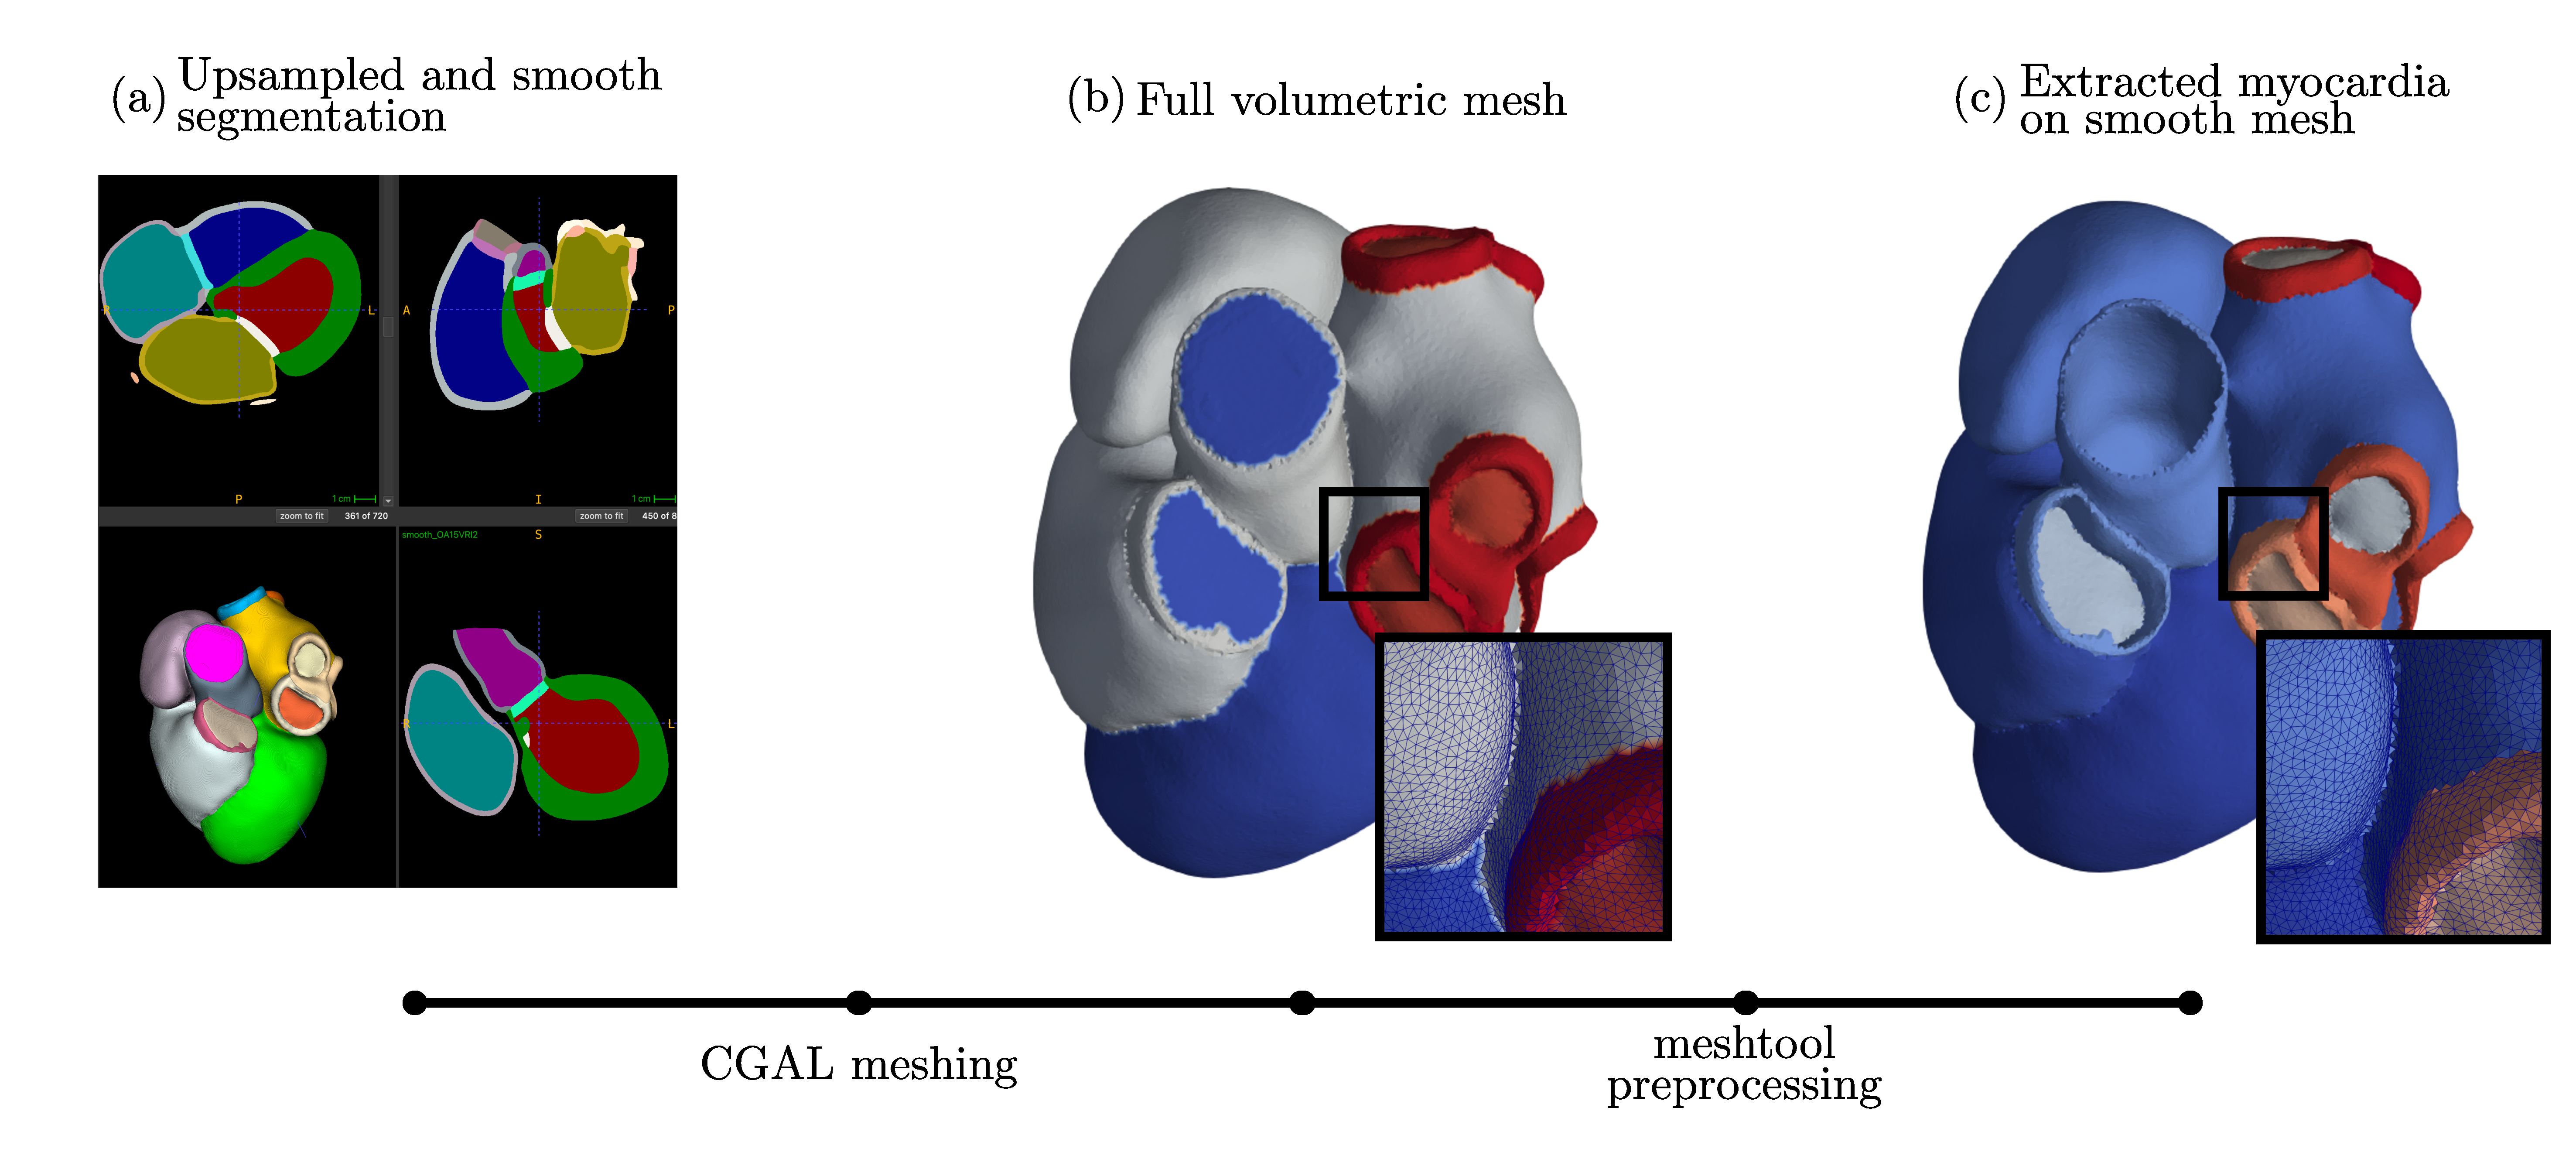
\includegraphics[width=\textwidth]{pics/methods-meshing.pdf}
    \caption{
        \textbf{Output of the meshing process from the smooth segmentation to the final working mesh.}
        (a) The upsampled and smooth segmentation. 
        (b) The mesh extracted from the segmentation using the CGAL meshing tool. 
        It contains all the blood pool and myocardium of the different structures.
        (c) The final mesh after the relabelling, cleaning, smoothing, and 
        extracting only the myocardia and valve planes. 
        Other outputs are created from this final process, such as specific endocardial and 
        epicardial surface meshes for the atria, which will be used later in the process.
    }
    \label{fig:methods-mesh}
\end{figure}

\subsection{Mesh Processing and Model Creation}\label{sec:model-creation}
The last stage of the pipeline included takes the smooth mesh and produces 
a model with fibre orientations, tagged with the different labels needed for the simulations.
This stage is run using CARP and meshtool~\cite{Neic2020-meshtool,carp-2003} along with 
the CEMRG Heartbuilder python library. 
Figure~\ref{fig:methods-model-creation} shows a visual overview of the model creation stage, 
which is described in detail below.

% Description of UVCs and ventricular fibres:
Universal Ventricular Coordinates (UVCs) are a system of coordinates that 
describe the geometry of the ventricles~\cite{bayer-2018-uvc}.
Additionally to the ventricles, UVCs are also calculated for the atria, 
to provide a system of coordinates defined on the volumetric mesh that facilitated 
the assignment of different tags within the mesh, and of boundary conditions for the 
pericardium.
To achieve this, 
the left and the right atria were treated as an upside down single ventricle,
\added[id=R1, comment={R1-Maj-2: Upside down ventricle citation}]{
    following the coordinate transformation approach described by Strocchi et al.~\cite{strocchi2020_simulating},
} 
with the apex manually placed between the two right pulmonary veins and behind the 
supervior vena cava, respectively. 

Atrial fibres are then assigned to the mesh by projecting a rule-based fibre 
field~\cite{labarthe2016_model}
onto the mesh using Universal Atrial Coordinates (UACs)~\cite{Roney2021-atlas}.
Ventricular fibres are then assigned to the mesh using a rule-based algorithm, 
described by~\cite{bayer2012_fibres},
which uses a series of Laplace solutions to assign the fibre direction.
% Description of UACs, atrial fibres, and mapping them to 3D:
UACs are a system of coordinates that describe the geometry of the atria~\cite{Roney2021-atlas}.
The atrial fibres, which originally are produced on surfaces, are then projected onto 
the 3D mesh, by assigning endocardial and epicardial fibres in the inner and outer 50\% 
across the thickness of the atria, respectively. 
From the UAC pipeline, which is run through a docker container, similar to the work 
by~\cite{solis-lemus2023_reproducibility}, the sino atrial node (\SAN) is also mapped
from the atlas. 

% Tags, electrodes and FEC layer
The mesh is tagged with the different labels needed for the simulations.
First, a region representing the fast-conducting Bachmann bundle is created, 
to simulate fast propagation of the electrical signal from the right to the left atrium. 
This is done using the UVCs defined on the atria.
The fast endocardial conduction layer (FEC) is also created at this stage, 
which is a thin layer of fast conducting tissue at the endocardium of the 
ventricles representing the Purkinje network.
In addition, to prevent unphysiological propagation from the atria to the ventricles and to 
control the atrioventricular delay, 
the atria and the ventricles were electrically isolated from each other by defining a 
layer on 
\replaced[id=R1, comment={R1-Min-2: Non-conduting typo fix}]{
    non-conducting
}{
    non-conduting
} 
tissue between the atrial and ventriclar myocardium.
Finally, the \SAN\ and the left and right ventricular fascicles are also created, 
Figure~\ref{fig:methods-model-creation}~(f.1, f.2, f.3). 
The SAN and fascicles are used to initiate electrical activation in the electrophysiology (EP) simulations. 
The left and right fascicles represent the first breakthrough from the Purkinje network into 
the myocardium to mimic the activation reported by the Durrer maps~\cite{durrer-1970-fascicles}. 
These locations are defined in UVCs based on~\cite{gillette_automated_2021}.

\paragraph{Mesh Quality Assessment}
\added[id=R2, comment={R2-3: Mesh quality assessment paragraph}]{
    We assessed the quality of all 50 volumetric meshes using the volume-based 
    distortion metric (\texttt{tet\_qmetric\_volume}) implemented in 
    meshtool~\cite{Neic2020-meshtool}, which quantifies element distortion relative to 
    an ideal tetrahedron. This metric is directly related to the determinant 
    of the Jacobian of the geometric map and is normalised to $[0, 1]$, where 
    0 corresponds to a perfect tetrahedron and 1 to a fully degenerate element.
}
\added[id=R2, comment={R2-3}]{
    Across all 50 meshes (mean $2.6 \times 10^6$ elements per mesh, range 
    $1.9$--$4.5 \times 10^6$), the mean element quality was $0.153 \pm 0.100$ 
    (mean $\pm$ SD across all elements in the cohort). The minimum quality per 
    mesh averaged $2.1 \times 10^{-4}$, indicating that even the worst elements 
    retained near-ideal geometry. No inverted elements (quality $> 0.99$) were 
    detected. Near-degenerate elements (quality $> 0.90$) were found in 28 of 
    50 meshes, comprising at most 9 elements per mesh ($< 0.0003\%$ of total 
    elements). These results confirm high geometric fidelity suitable for 
    finite element analysis.
}

\begin{figure}[hbpt]
    \centering
    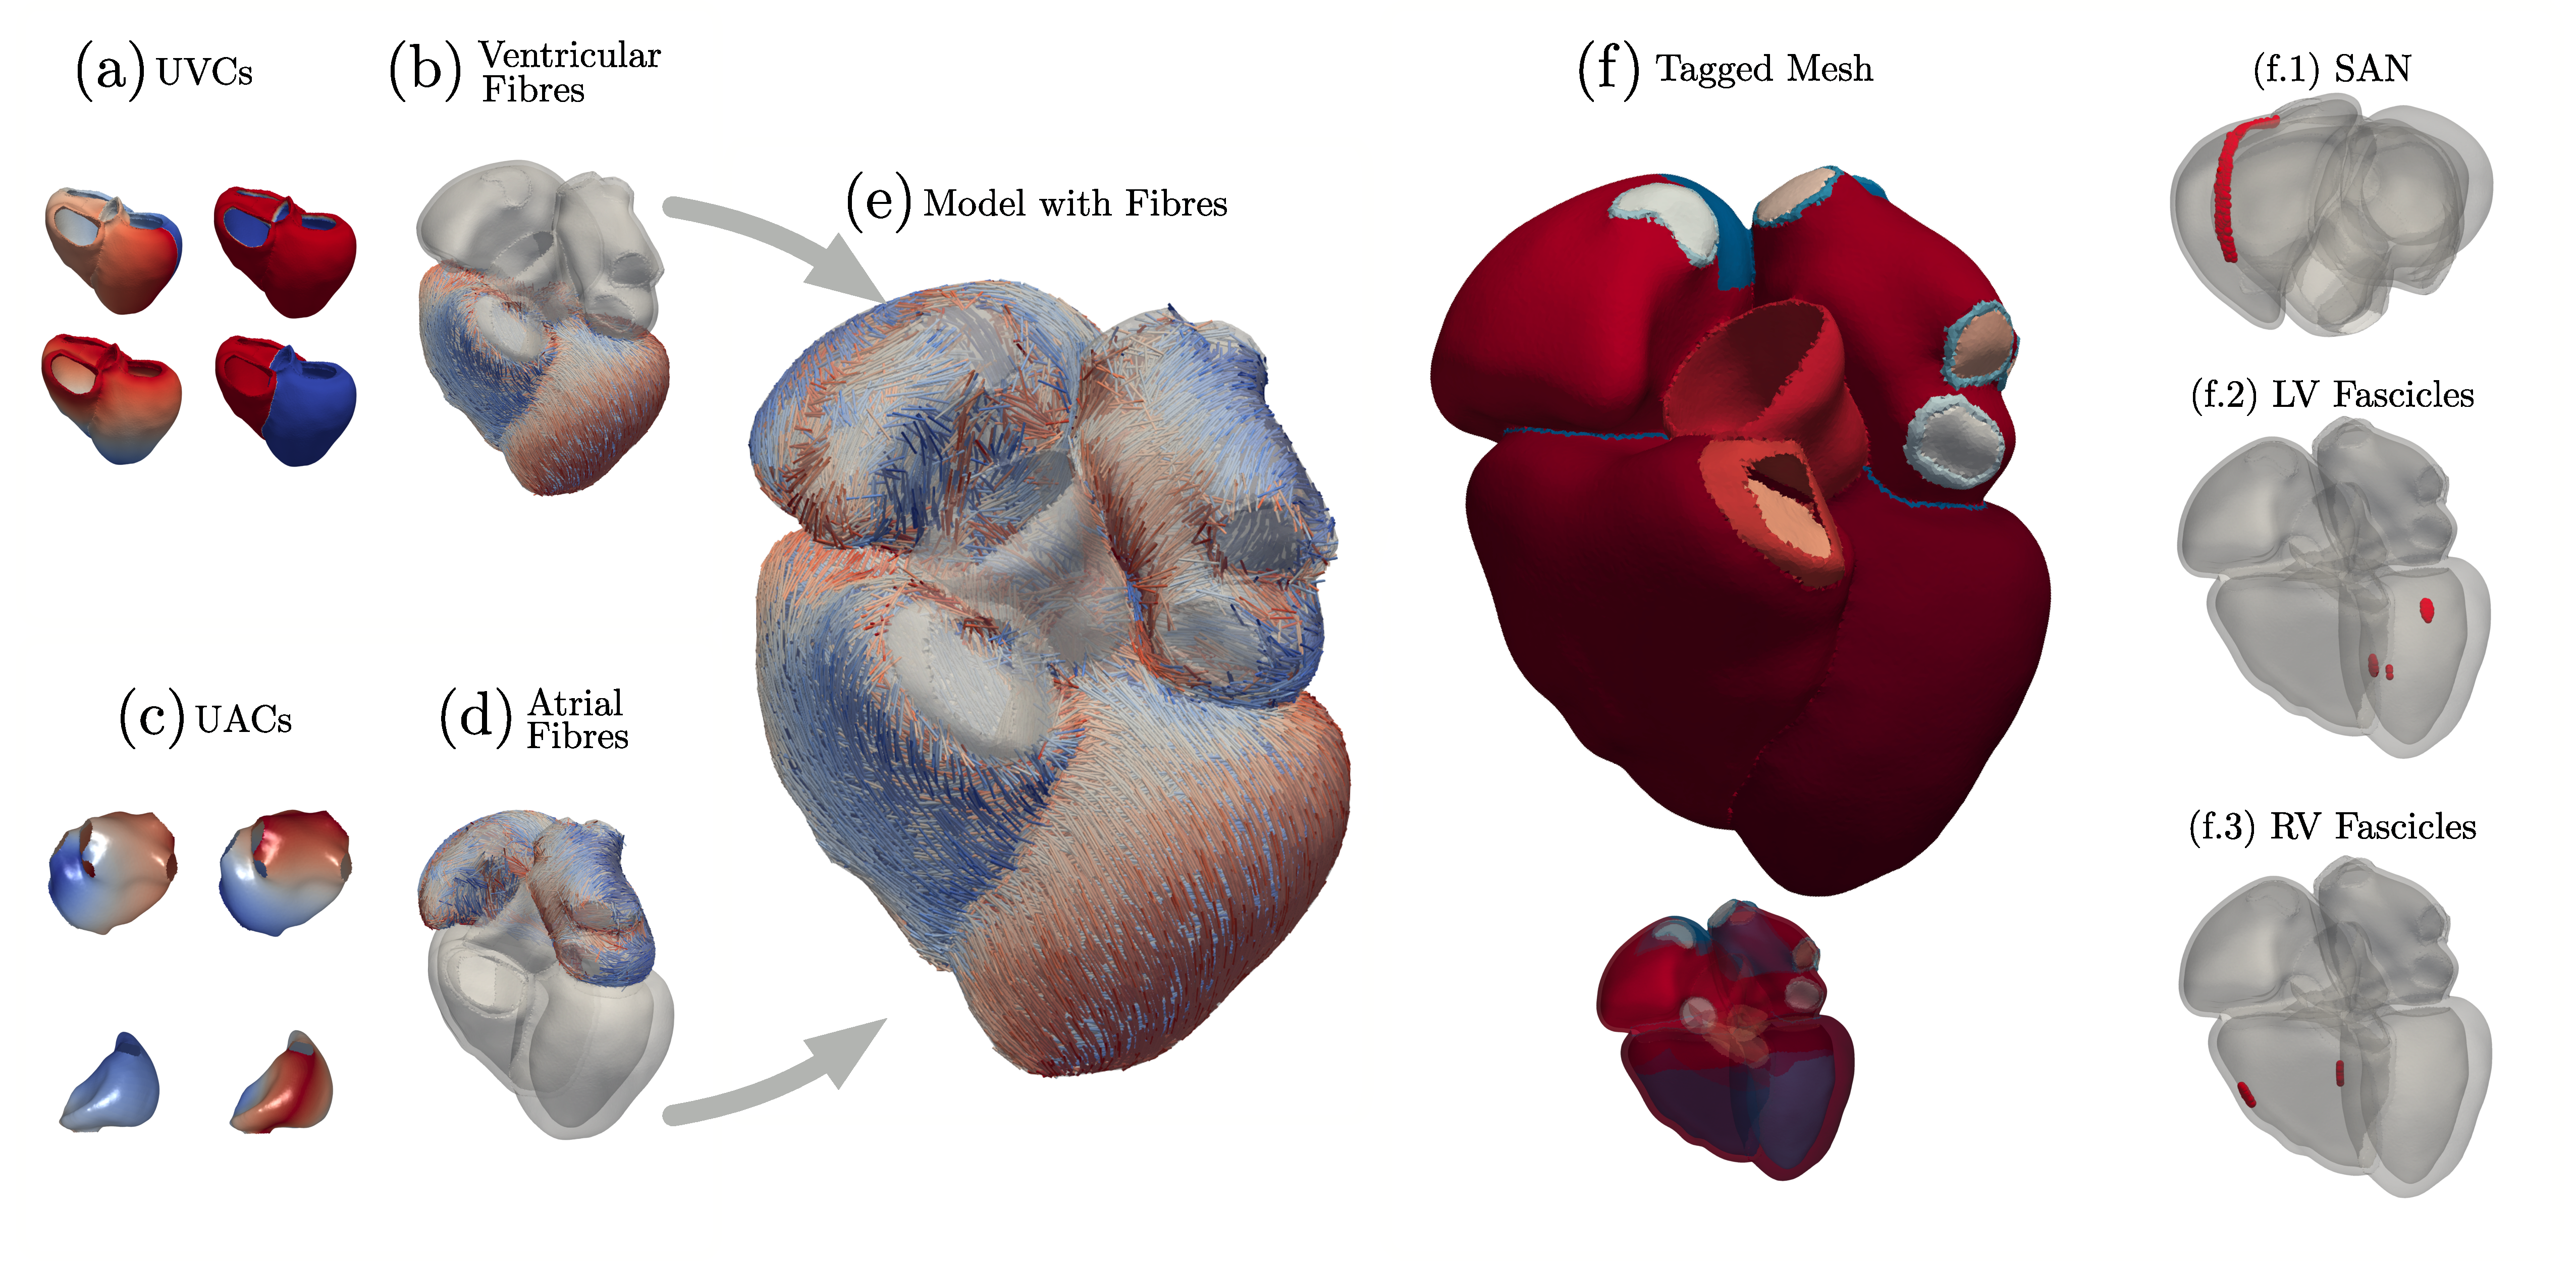
\includegraphics[width=\linewidth]{pics/methods-model-creation.pdf}
    \caption{
        \textbf{Model creation stage. }
        % Description of UVCs and ventricular fibres:
        Universal Ventricular coordinates (a) are calculated from the mesh, then used to assign 
        the fibre direction (b) using a rule-based algorithm~\cite{bayer2012_fibres}.
        % Description of UACs, atrial fibres, and mapping them to 3D:
        Universal Atrial coordinates (c) are calculated from the mesh, then used to assign
        the fibre direction (d) using a projection from an atlas~\cite{Roney2021-atlas}.
        The atrial fibres, which originally are produced on surfaces, are then projected onto the 3D
        mesh.
        % Tags, electrodes and FEC layer 
        The fibres from the ventricles and atria are then assigned to the model (e).
        The final mesh is tagged with the different labels needed for the simulations (f).
        The fast endocardial conduction layer (FEC) is also created at this stage (f~-~bottom),
        which is a thin layer of fast conducting tissue at the endocardium of the ventricles.
        Finally, UVCs and UACs are used to create the sino atrial node (\SAN, f.1),
        the left ventricle fascicles (f.2) and right ventricle fascicles (f.3).
    }
    \label{fig:methods-model-creation}
\end{figure}

\subsection{Simulations}\label{sec:simulations}

We performed EP and mechanics simulations on all the models. 
Simulations were run with a fixed set of parameters to assess the impact 
anatomical differences would have on the outputs. 
These simulations also served as an additional quality check for the meshes, 
to ensure the models could be used to run electromechanics simulations. 

\added[id=R2, comment={R2-4: Spatial alignment protocol}]{
    Each patient-specific mesh was simulated in its native 
    coordinate system without spatial registration to a common anatomical 
    reference frame. Comparisons between models were performed on scalar 
    outputs (chamber volumes, total activation times) that are invariant 
    to rigid transformations. Universal Ventricular Coordinates 
    (UVCs)~\cite{bayer2018} provide normalized transmural and apicobasal 
    coordinates for regional functional analysis independent of absolute 
    spatial positioning.
}

The EP simulations were started at the \SAN, defined in Section~\ref{fig:methods-model-creation}. 
The ventricular endocardial electrodes (fascicles) were also activated simulating the early activation 
sites~\cite{Gillette-2021-dt}. 
The reaction-eikonal model~\cite{neic-2017-electrograms} was solved to compute the activation 
times at each node. 
A conduction velocity of $1$ m/s was used at the myocardial tissue, with a 
$40\%$ anisotropy cross-fibre, and a 
$6$-fold speed in the fast activation regions~\cite{lee-2019-fec}. 
As output, the total activation time of each ventricle, of both ventricles and both atria were extracted.

To test how differences in anatomy impacted simulation predictions,
we performed inflation simulations to evaluate the mechanical behaviour of the models.
Briefly, increasing pressure is applied at the endocardium of each chamber until a 
maximum established pressure of  
% 0.93~kPa for the left chambers (\LV\ and \LA) and
7~mmHg for the left chambers (\LV\ and \LA) and
% 0.466~kPa for the right chambers (\RV\ and \RA) 
3.5~mmHg for the right chambers (\RV\ and \RA) 
is reached.
The myocardium was modelled as an transversely isotropic hyperelastic material using the 
Guccione's material law~\cite{Guccione-1991-material-props}, 
while the rest of the cardiac structures were modelled as isotropic hyperelastic materials using a 
NeoHookean material law~\cite{faulkner-1972-nearly}. 
Mechanics simulations were run with the same boundary conditions as the work by~\cite{strocchi2023_cell}, 
which can be consulted in the Supplementary Material.

Simulations were run to assess the impact of anatomical differences on the outputs and to serve as 
a quality chech for the meshes. 
All simulations were run with CARP~\cite{carp-2003}. 
The EP simulations were run in a $20$-core workstation, 
while the inflation simulations were run in the UK national supercomputer ARCHER2, using $512$ cores.

% \subsection{Model Quality Control and Validation Tests}
Model outputs obtained from the simulations are listed in Table~\ref{tab:measurements},
along with a brief descripton. 
The 18 measurements are grouped into four categories:
activation times (4 outputs),
inflated volume (4),
volume change (absolute 4, and normalised 4), and
volume ratios (2).
The absolute volume change ($\deltaVol{}$) is calculated as the difference between the maximum and minimum volume
during the inflation simulation.
For simplicity, we refer to inflated volume as volume throughout the manuscript.
The normalised volume change ($\deltaVolNorm{}$) is calculated as the percentage of change in volume,
and the volume ratio is calculated as the ratio between the left and right volumes, 
this was calculated for the ventricles and the atria. 
The Total Activation Time ($\TAT{}$) is the time it takes for the electrical signal to propagate
through the entire chamber.

\begin{table}[hbpt]
    \centering
    \caption{
        \textbf{Model outputs obtained from the simulations.}
        The subscript $x$ refers to the chamber, which can be left ventricle (LV),
        right ventricle (RV), left atrium (LA), or right atrium (RA). 
    }
    \vspace{1em}
    \begin{tabular}{lll}
    \hline
    Measurement              & Symbol                           & Calculation / Definition                                                                                  \\
    \hline
    Total Activation Time    & $\TAT{x}$                        & All chambers, ventricles, and atria                                \\
    (Inflated) Volume        & $\VOL{x}$                        & All chambers                                                     \\
    Volume Change            & $\deltaVol{x}$                 & Maximum minus minimum volumes  \\
    Normalised Volume Change & $\deltaVolNorm{x}$            & Percentage of change in volume                  \\
    Volume Ratio             & $\frac{L}{R}$ & Ratio of left and right volumes \\                            
    \hline 
    \end{tabular}    
    \label{tab:measurements}
\end{table}

\paragraph{QRS duration.} 
Since the simulations do not include a torso, the comparison cannot be made directly 
with the QRS duration measured in the ECGs. 
Instead, we used the total activation time in the ventricles as a surrogate 
for QRS duration and compared it between the different groups.

\paragraph{Total Activation Time in the Atria.}
This parameter has emerged as a key marker of atrial remodeling and is associated with \HF\ 
progression and complications~\cite{sanders-2003-atrialremodelling,buck-2008-crt}.
We assessed the total activation time in the atria, comparing it between the different groups.

\subsection{Statistical tests and comparison of volume to clinical literature}
We performed a multi‐step statistical analysis of our cardiac dataset.
First, we computed descriptive statistics (mean $\pm$ SD) for all core metrics (volumes and activation times)
stratified by sex, condition (\HF vs. control), and subtype (\HFN vs. \HFW). 
% To assess mesh‐size validity, we calculated Pearson correlations between mesh element counts and activation times.
Differences between narrow and wide QRS durations are only explored qualitatively, as the number 
of cases in each group is low. 

\paragraph{Effect sizes and statistical significance.}
% You want to see if there's a difference in an outcome (e.g., a heart metric) depending on:
To assess the differences in the outcomes, we used a two-way ANOVA to test the effects of 
Sex, Condition, and their interaction.
We followed up significant ANOVA results in the interactions with post-hoc pairwise comparisons 
using Tukey's method, 
and calculated Cohen's $d$ effect sizes~\cite{cohen-2013-statistical} for each comparison.
If the interaction was not significant, we performed marginal comparisons
between \HF\ and controls, or male and female groups, across all cases.
% ADJUST FOR MULTIPLE COMPARISONS
P‐values were corrected for multiple comparisons using the Benjamini–Hochberg 
false discovery rate~\cite{Benjamini1995ControllingTF}. 
Effect sizes are reported as Cohen's $d$, 
using Gignac's expanded criteria~\cite{gignac-2016-effects},
where $d<0.5$ is small, 
      $0.5<d<0.8$ is moderate, 
      $0.8<d<1.2$ is large, 
  and $d>1.2$ is very large.
% Finally, we visualized group distributions via boxplots with overlaid swarm plots, and
% summarized effect sizes in forest plots. 

To externally validate the models, 
we compared different outputs from the pipeline % and from simulations and  
linked them to a clinically relevant metrics.

\paragraph{Left atrial and left ventricular volume.} 
Left atrial volume is a predictor of outcome in patients with chronic \HF, 
independently of their symptoms, age, or \LV\ function~\cite{rossi-2007-lav}. 
\LV\ volume is a key prognostic factor in \HF, 
as it is associated with the severity of the disease and the risk of 
adverse events~\cite{kasa-2024-lv_volume,ito-2021-lv_volume}.
We assessed the left atrial volume ($\VOL{LA}$) and \LV\ volume ($\VOL{LV}$) in the models, 
comparing between the different groups.
For $\VOL{LV}$, we compared measurements from our cohort with reference values from the UK biobank 
(UKBB)~\cite{petersen-2017-reference}, which defines normal ranges for left and right ventricles
in males and females. 
Outside the normal ranges, we considered the volumes to be abnormal,
and therefore indicative of \HF\ or other cardiac conditions. 

% \paragraph{Left-ventricular and left-atrial chamber stiffness.}
% Stiffness can be approximated in a shell with constant thickness using Laplace's law.
% It is measured as the ratio between change in pressure and change in volume. 
% In our simulations, as the pressure is always the same for all cases, 
% the change in volume becomes a surrogate for stiffness. 
% It has been reported that patients  with \HF\ show increased 
% \LV\ chamber stifffness~\cite{zile-2004-stiffness,aurigemma-2006-stiffness}.
% Similarly, \LA\ chamber stiffness has shown to predict mortality and 
% hospitalisation~\cite{Carpenito-2021-la-stiffness,kim-2023-la-stiffness}. 
% Because stiffer chambers deform less under the same pressure, increased volume change ($\deltaVol{LV}$) 
% indicates reduced chamber stiffness. 
% Therefore, if chamber stiffness is reduced in the heart failure group, 
% we expect to observe a larger volume change compared to controls.



% 